\documentclass[conference]{IEEEtran}
\IEEEoverridecommandlockouts
% The preceding line is only needed to identify funding in the first footnote. If that is unneeded, please comment it out.
\usepackage{cite}
\usepackage{amsmath,amssymb,amsfonts}
\usepackage{algorithmic}
\usepackage{graphicx}
\usepackage{textcomp}
\usepackage{xcolor}
\usepackage[utf8]{inputenc}
\usepackage[T1]{fontenc}
\def\BibTeX{{\rm B\kern-.05em{\sc i\kern-.025em b}\kern-.08em
    T\kern-.1667em\lower.7ex\hbox{E}\kern-.125emX}}
\begin{document}

\title{Simulação de Desastre - Sistema Multiagentes  Trabalho de IA\\
}

\author{\IEEEauthorblockN{Lucas Vieira, Lucas Martins, Victor Henrique Ribeiro}
\IEEEauthorblockA{\textit{UNESP Júlio de Mesquita Filho} \\
\textit{ Ciência da Computação Noturno, 2018}\\
Rio Claro, Brasil\\}
}

\maketitle

\begin{abstract}
Um breve estudo sobre uma ferramenta de simulação de desastre, e programação de multiagentes
\end{abstract}

\begin{IEEEkeywords}
RescueCup, Multiagentes, Inteligência Artificial, Simulação.
\end{IEEEkeywords}

\section{Introdução}
A Inteligência Artificial consiste na criação de softwares inteligentes que tem a capacidade simular a capacidade humana de raciocinar, tomar decisões e resolver problemas. Suas aplicações são muitas e aqui iremos ver uma aplicação de simulação de desastre, que consiste em desenvolver a melhor estratégia, programaticamente para atuar em uma situação de desastre.

A inspiração para a criação do simulador, ocorreu em 1995 onde na cidade de Kobe no Japão, ocorreu um terremoto que matou mais de 6 mil pessoas. Isso levou uma equipe a iniciar uma pesquisa onde criaram um simulador de um terremoto em uma cidade, a razão disso foi criar uma ferramenta, para criar estratégias de resgate em situações como essa, sendo possível avaliar a eficiência das estratégias baseado numa pontuação.

Essa ferramenta é utilizada na competição anual Robocup Rescue Simulation League, onde equipes de universidades do mundo todo, criam estratégias para  a abordar o problema, e aqui neste trabalho vai ser nosso desafio, desde a compreensão das ferramentas utilizadas e a programação dos agentes para a atuarem na simulação.

\section{Ferramentas}

\subsection{Robocup Rescue Simulation Server}

Este software trata-se do centro do nosso estudo, ele é composto por vários simuladores que comunicam entre-si e com os agentes, tudo através de um simulador de Kernel que gerencia toda essa interação.

\begin{figure}[htbp]
\centerline{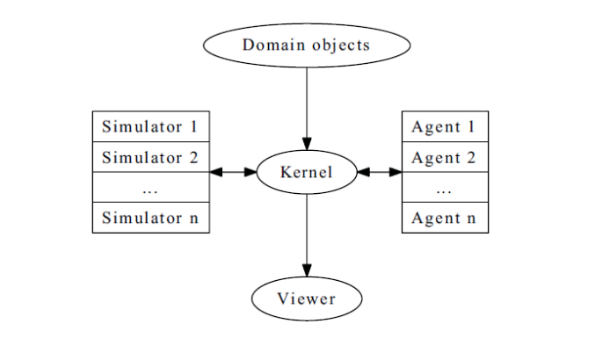
\includegraphics[scale=0.4]{fig1.png}}
\caption{Arquitetura do RoboCup Rescue Agent Simulation\cite{b1}}
\label{fig1}
\end{figure}

O software é composto 6 simuladores:
\begin{itemize}
\item \textit {Clear Simulator} - Responsável pela remoção de bloqueios das estradas. 
\item \textit {Collapse Simulator} - Responsável por gerenciar os danos estruturais dos prédios para criar bloqueios.
\item \textit {Ignition Simulator} - Realiza o princípio de incêndio nos prédios durante a simulação.
\item \textit {Fire Simulator} - Responsável por espalhar o fogo entre os edifícios.
\item \textit {Traffic Simulator} - Simulador responsável pelo movimento das entidades humanas.
\item \textit {Misc Simulator} - Responsável pelo dano de humanos e estruturas.
\end{itemize}

Na arquitetura do ambiente, como visto na Fig 1, ainda estão os objetos da cena, que estão armazenados em um arquivo com a extensão .gml, onde estão todas os prédios e ruas do mapa. O "Viewer" seria uma visualização gráfica do estado do sistem, onde estão sendo atualizados os agentes e estruturas no ambiente. 

Já os agentes são responsáveis pelas ações que alteram o ambiente, onde enviam suas ações para o kernel, ele gerencia a comunicação com o determinado simulador responsável pela ação e atualiza o "Viewer" de acordo com a situação atual do ambiente, mais detalhes serão explicados na seção sobres os Agentes e o ambiente.
\subsection{Eclipse - Linguagem Java}
A própria ferramenta tem bibliotecas e samples, todas são feitas em Java, portanto foi facilmente a linguagem escolhida para o trabalho. No Robocup Rescue a atuação das equipes que participam do evento é na formulação de estratégias entre os agentes e de agentes com o ambiente. Portanto o desafio é gerenciar todas essas variantes programaticamente. 
O código é composto de classes auxiliares e classes do código dos Agentes. A função do eclipse é compilar este código e carregar os agentes ao Simulation Server, onde após isso os algoritmos serão executados no kernel do simulador, por fim atuando na simulação.

\subsection{JOSM Editor}
\textit {JOSM Editor - Java OpenStreetMap Editor} é a ferramenta utilizada para criar o nosso ambiente, que é o mapa que contém prédios e ruas. É uma ferramenta de software livre, onde é possivel selecionar uma área em qualquer lugar mapa-mundi e obter sua representação por meio de objetos como prédios, ruas, jardins, estacionamentos, etc.

\begin{figure}[htbp]
\centerline{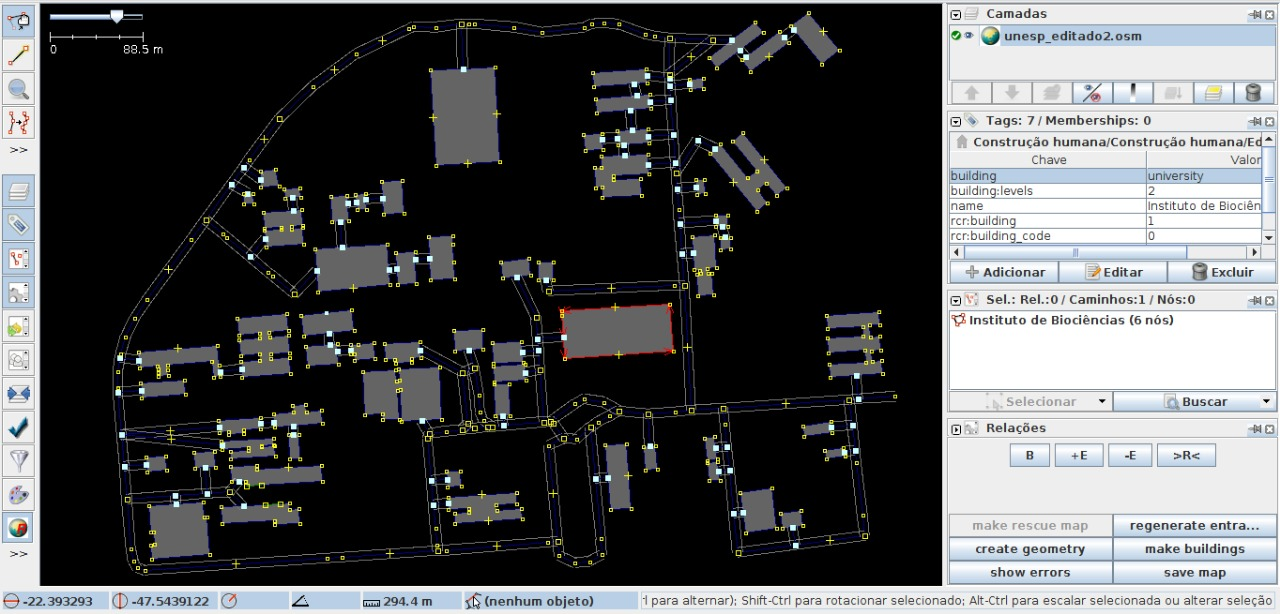
\includegraphics[height=3.3cm]{fig3.jpeg}}
\caption{Imagem do mapa da UNESP criado pelo JOSM \cite{b2}}
\label{fig2}
\end{figure}

No nosso projeto, utilizamos a ferramenta para criar um mapa da UNESP Júlio de Mesquita Filho como mostrado na Figura 2, houve a necessidade de retirar alguns detalhes do mapa, para que o simulador consiga utilizar corretamente os objetos do mapa, isso acontece pois o JOSM não gera um arquivo compátivel com o mesmo, sendo necessário realizar uma conversão para o formato .gml, ao realizar essa conversão, alguns detalhes são perdidos ou alguns objetos precisam ser editados para realizar com sucesso a conversão.

\section{Ambiente - Entidades do Ambiente}
O ambiente é o lugar onde os agentes e simuladores interagem, onde ocorre a simulação. E que no caso deste projeto é representado por um mapa, onde há agentes, prédios e ruas.
\subsection{Blockade}
Blockades ou bloqueios são entidades que obstruem o caminho nas vias, portanto dificultando ou até mesmo impedindo a movimentação dos agentes.
Eles são gerados pelo \textit{Collapse Simulator} de acordo com o dano aos edifícios, simulando assim detritos e prédios entrando em colapso em uma situação de desastre. Os bloqueios possuem certas propriedades como: posição, custo de reparo, formato, coordenadas e arestas.

\subsection{Área}
Áreas são considerados os prédios e ruas do mapa, os bloqueios acontecem em ambos, mas somente nas ruas os bloqueios são visíveis. Programaticamente as áreas possuem certas propriedades,como: bloqueios na área, arestas da área, lista de áreas vizinhas e coordenadas da área no mapa.
\subsection{Buildings - Localizações Chave}
Há quatro localizações chave no simulador, e essas são:
\begin{itemize}
\item \textit {Refuge} - Refúgio para os civis.
\item \textit {Ambulance Central} - Central de comunicação dos Médicos
\item \textit {Fire Station} - Central de comunicação dos Bombeiros
\item \textit {Police Office} - Central de comunicação da Polícia
\end{itemize}
Mais detalhes sobre comunicação serão descritos posteriormente neste documento.


\section{Agentes}
Os agentes são os atores do simulador, que interagem com o sistema e comunicam entre si. Nesta seção serão explicados as ações e funções de cada um.
\subsection{Civillians}
Os civis são os agentes que devem ter seu caminho facilitado por outros agentes até o refúgio, eles são responsáveis por grande parte da pontuação final, sendo a maior prioridade na simulação.
\subsection{Police Force}
A polícia tem como objetivo limpar os blockades, ou seja, facilitar o caminho de todos os agentes no ambiente.
\subsection{Fire Brigade}
Os bombeiros tem como função apagar incêndios em prédios, eles carregam uma certa quantidade de 'água', que após ser usado deve ser reabastecido em um \textit{Refuge}.
\subsection{Ambulance Team}
Os médicos são os agentes que resgatam outros agentes e levam ao refuge, eles também salvam agentes enterrados e carregam no máximo um agente.
\subsection{Central Agents}
Representados como localizações chave, \textit{Ambulance Centers}, \textit{Fire Stations} e \textit{Police Offices}. Tem como única função realizar a comunicação via rádio com os agentes.

\section{Percepção e Comunicação}

\subsection{Percepção - Lines of sight}
A percepção de cada agente é representada por linhas no simulador, ou seja, aonde as linhas conseguem atingir é o que o agente consegue "enxergar" o que está acontecendo no ambiente, como representado na Figura 3.
\begin{figure}[htbp]
\centerline{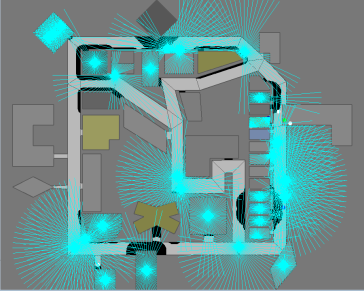
\includegraphics[scale=0.6]{fig2.png}}
\caption{Lines of Sight - Representação das linhas de visões dos agentes \cite{b1}}
\label{fig3}
\end{figure}
Por exemplo, se um agente vê um bloqueio e o mesmo sai do seu campo de visão, mesmo se o bloqueio for limpo, para o agente ainda vai haver um bloqueio aonde ele passou. Portanto a sua visão atualiza seu conhecimento do ambiente.

\subsection{Comunicação}
A comunicação auxilia na tomada de decisões dos agentes, atualizando as percepções de mundo entre agentes.

Existem dois tipo de comunicação no simulador:
\begin{itemize}
\item \textit {Direct communication} - É a simulação de uma comunicação oral humana,portanto é emitida de um agente e outro agente só a recebe se estiver dentro do raio de alcance do emissor.
\item \textit {Radio communication} - comunicação por radio realiza a interação das localizações chave para com os agentes, portanto ela atinge todos os agentes de uma mesma classe por todo o mapa.
\end{itemize}

Ambos os tipos de comunicação estão suscetíveis a falhas, em ambos os casos há a possibilidade de \textit{dropout} que é a a falha de um agente em receber a mensagem. Mas no caso de \textit{radio communication}, há outra falha possível que seria a de \textit{failure}, onde um agente recebe a mensagem mas ela vem vazia.

\section{Programação de Agentes}
A programação de agentes envolve a utilização de conceitos que imitam a atuação humana em situações de desastre. Por exemplo, ouvir algum civil pedindo por socorro, envolve passar informações valiosas para agir no ambiente para outros agentes. E principalmente agir em prol do objetivo, que é o resgate de civis.
Lembrando que os agentes só podem realizar uma ação por 'turno', seja essa andar, resgatar, etc. Já a comunicação é permitida que seja uma ação adicional, portanto pode se mover e se comunicar em um 'turno', por exemplo.
\subsection{Civis}
Os civis tem o código provido pelo próprio simulador, eles traçam um caminho para o refúgio, se esse caminho tiver obstruído ele espera por socorro. Ele também chama por socorro para agentes a sua volta receberem a sua posição.
\subsection{Police Force}
Esse agente age mediante a 3 estados: \textit{AVAILABLE}(Disponível), \textit{WALK}(Andando) e \textit{CLEAR}(Limpar). A principal função de um policial é limpar as vias do ambiente, portanto foi priorizado o agente estar se movendo sempre que disponível, com o objetivo de encontrar mais blockades para limpar.

Na ação \textit{WALK}, o agente anda de 2 formas, uma seria randomicamente, através de uma função que procura caminhos possíveis e sorteia um para o agente andar, assim encontrando possíveis blockades. A outra forma de andar seria direcionada a um objetivo, que no caso do policial seria um \textit{blockade}, dessa maneira quando é encontrado um bloqueio, e o agente entra em estado \textit{CLEAR}, o mesmo vai andar em direção ao bloqueio buscando eliminá-lo.

A ação \textit{CLEAR}, que é a principal função do policial, consiste no momento em que for detectado um \textit{blockade}, o mesmo deve ser limpo com a função \textit{sendClear}, que com o envio das informações do blockade, realiza a limpeza do bloqueio. A complexidade dos bloqueios é algo definido pelo o simulador 'collapse', portanto o \textit{sendClear}, que utiliza o simulador 'clear'.Dependendo da complexidade do bloqueio, a limpeza não é instantânea, sendo necessário várias chamadas da função \textit{sendClear} para eliminar o bloqueio por completo.

A primeira ação do policial é tentar limpar os bloqueios no caminho do \textit{refuge}, pois somente lá os civis estão a salvo. Logo após essa ação, todos os bloqueios que estão próximos serão limpados, porém dois políciais tentando limpar o mesmo bloqueio não acelera o processo, por causa disso, cada policial assume a responsabilidade de um bloqueio para que outros agentes não tentem limpa-lo.

Caso não haja nenhum bloqueio próximo, o agente tenta verifica se ele deixou algum bloqueio pra trás, verificando a lista de bloqueios que ele assumiu responsabilidade, caso ele encontre algum bloqueio existente nessa lista ele se direciona para limpa-lo. Caso contrário ele faz movimentos aleatórios até encontrar novos bloqueios.
\subsection{Ambulance Team}
As ambulâncias tem a programação para sempre andar de prédio em prédio em busca de sobreviventes, a função deste agente é o resgate de civis e outros agentes soterrados. 
Após achar um civil, o agente deve leva-lo até o \textit{refuge}, os agentes gastam um tempo grande enquanto estão tratando civis, esse tempo é calculado pela função \textit{sendRescue} que é uma das bibliotecas do simulador.

Como não podemos melhorar o tempo de tratamento, o foco é a melhor distribuição das ambulâncias em busca de vítimas, como por exemplo no caso de quando 2 ou mais ambulâncias estão tratando da mesma vítima, são dois agentes alocados a uma tarefa, e não torna mais rápida, e sim inútil a presença de mais que um agente. Portanto o que fizemos foi um cadastro de vítimas, com a classe \textit{AmbulanceHelper}. É montado uma lista com os agentes alocados a determinadas vítimas e somente o responsável pela vítima vai conseguir realizar o tratamento, enquanto outros agentes que passarem por ali irão, reconhecer que a vítima já tem um agente alocado a ela e irão seguir em frente em busca de mais vítimas.

Como os agentes são executados em \textit{threads}, ou seja, em paralelo, ocorre uma concorrência pela vítima e portanto o agente que conseguir manter-se com aquela vítima é o único que irá tratá-la.

Uma pequena alteração que surtiu efeito, foi que, quando as ambulâncias tinham seu caminho bloqueado ao prédio, elas ficavam esperando o bloqueio ser removido para seguir ao prédio não explorado, isso acaba gerando agentes ociosos a espera de ação de outros agentes, tornando o agente não pró-ativo. Portanto a cada 3 \textit{steps} que o agente fica na mesma posição sem andar, o que provavelmente é um blockade, ele anda  aleatoriamente até encontrar um civil necessitando de ajuda. Só após isso ele volta procurar prédios inexplorados. 
\subsection{Fire brigade}
Os bombeiros precisam apagar os incêndios o mais rápido possível para que não se alastre entre os prédios próximos, por causa disso eles ficam andando entre os prédios e verificando o estado dos mesmos, caso detectem algum prédio em chamas no seu alcance, eles tentam apagar o fogo, caso contrário, tentam se dirigir para uma posição mais próxima, sendo possível apagar o fogo.

Uma dificuldade é que os agentes possuem uma quantidade limitada de água, sendo necessário se dirigir até o refúgio para reabastecer, isso faz com que as vezes demore para apagar determinados incêndios dependendo da posição em relação ao refúgio.

Diferente dos outros agentes, dois bombeiros agindo sob um mesmo incêndio aumenta a velocidade em que ele é apagado, por isso é permitido a cooperação entre os próprios bombeiros para apagar o fogo.

\section{Resultados Obtidos}
O simulador quando iniciado, possui uma pontuação inicial, baseada no numero de prédios e civis, esta pontuação nunca aumenta, ela apenas diminui ao longo da simulação, cada civil morto ou prédio destruido, diminui uma quantidade da pontuação geral.

Foram realizados alguns testes com os agentes de exemplo que acompanham o simulador, os mesmos não possuem nenhum comportamento organizado e simplesmente ficam executando as ações no seu ambiente ao redor.

Nos nossos testes a simulação rodou durante 300 \textit{steps}, a pontuação inicial era de 38.94, possuindo um total de 38 civis. 
\begin{figure}[htbp]
\centerline{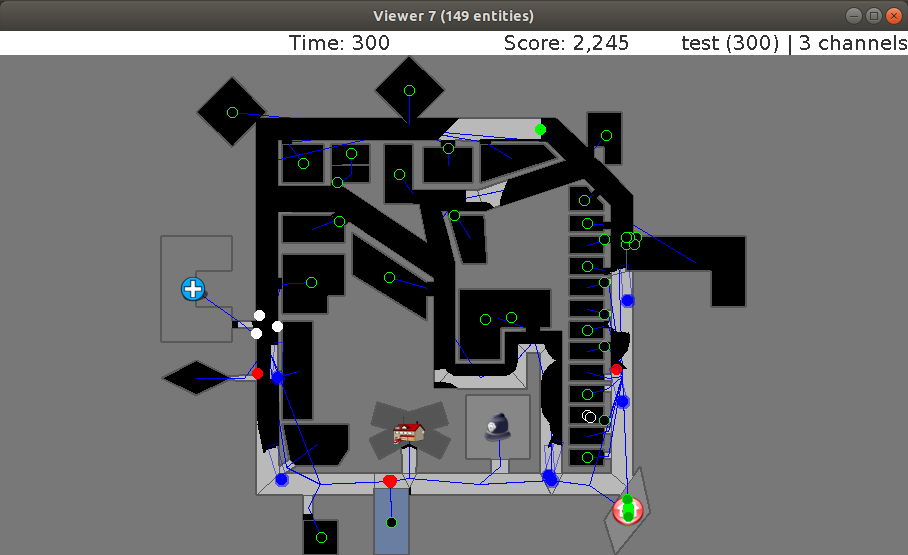
\includegraphics[scale=0.27]{fig4.png}}
\caption{Simulação com os agentes \textit{Sample}}
\label{fig4}
\end{figure}

O sample teve esta baixa pontuação devido ao fato que muitos agentes ficavam parados depois de um tempo, os policiais ficavam tentando limpar bloqueios mas nunca saiam do lugar e dessa forma, quase nenhuma via estava disponivel para os outros agentes.

Após pensar em algumas estratégias para resolver os problemas do sample, foram resolvidos vários problemas que diminuiam a pontuação no geral. Primeiramente os policiais limpam o caminho até o refúgio permitindo os civis livres a correrem para o mesmo e ficarem a salvo, além disso os policiais e médicos, dividiram as tarefas, onde cada agente se torna responsável por um civil ou bloqueio, dessa forma, tornando mais rápida as ações dos mesmos. Por fim os bombeiros ficam caminhando entre os prédios em busca de prédios em chamas, diminuindo as chances do fogo de alastrar entre os prédios.

\begin{figure}[htbp]
\centerline{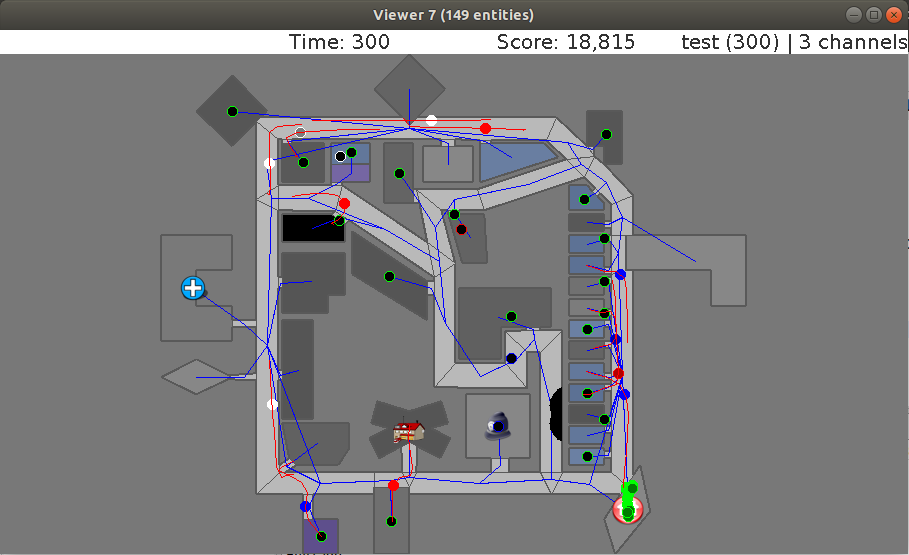
\includegraphics[scale=0.27]{fig5.png}}
\caption{Simulação com os agentes \textit{Sample}}
\label{fig5}
\end{figure}

Dessa forma, coordenando os agentes entre si e analisando os principais problemas enfrentados pelos agentes, conseguimos uma pontuação máxima de 18.815, sendo esta 838.08\% maior que a pontuação obtida na versão inicial.

\section{Conclusão}
Neste sistema multiagente muitos dos problemas poderam ser resolvidos analisando como os agentes devem se comportar sozinhos e como se comportar em relação aos outros agentes. A maior dificuldade provavelmente foi como coordenar os agentes para que eles consigam cooperar entre si de uma forma que todos executem suas ações da melhor forma.

Não existe uma solução perfeita, pois a simulação é sempre aleatória e dependendo do ambiente, os agentes se comportam de maneira diferente, podendo gerar resultados diversos com os mesmos agentes.

Dessa forma nossa estratégia de dividir as tarefas foi a melhor solução encontrada para melhorar o desempenho dos agentes, além de definir as possíveis ações que ele pode realizar mediante ao ambiente atual, sendo versátil para realizar diferentes ações.

Diferentes estratégias podem ser adotas para melhorar ainda mais nossa pontuação, como a ultilização dos centros para coordenar os agentes e a implementação de diferentes algoritmos de caminhos.

\begin{thebibliography}{00}
\bibitem{b1} Annibal B. M. da Silva, Luis G. Nardin and Jaime S. Sichman, ``Robocup Rescue Simulator Tutorial,'' Laboratório de Técnicas Inteligentes - Escola Politécnica da USP, São Paulo - SP.
\bibitem{b2} Alan D. Barroso, Felipe Santana e Victor Lassance, "Tutorial for the Creation of a Robocup Rescue Simulator Map", Escola Politécnica da USP, São Paulo - SP.

\end{thebibliography}

\end{document}
